\documentclass[12pt,a4paper,reqno]{amsart}

% language
\usepackage[greek,english]{babel}
\usepackage[utf8]{inputenc}
\usepackage{alphabeta}

% change default names to greek
\addto\captionsenglish{
    \renewcommand{\contentsname}{Περιεχόμενα}
    \renewcommand{\refname}{Βιβλιογραφία}
    \renewcommand{\datename}{Ημερομηνία:}
    \renewcommand{\urladdrname}{Ιστοσελίδα}
}

% math 
\usepackage{amsmath,amsthm,amssymb,amscd}

% font
\usepackage[cal=euler]{mathalfa}
\usepackage{libertinus-type1}
% \usepackage{txfonts} % for upright greek letters
\usepackage{bm} % for bold symbols
\usepackage{bbm} % for the simply-looking bb symbols

% miscellaneous 
\usepackage{changepage} %for indenting environments
\usepackage{csquotes} % example: \textcquote{}
\usepackage{blkarray}
\setcounter{MaxMatrixCols}{20} % default for pmatrix is 10!!
\usepackage{ytableau}
\usepackage{array} %needed to increase the vertical length in a tabular

% drawing
\usepackage{tikz,tikz-cd}
\usetikzlibrary{shapes.misc, patterns, matrix, calc, intersections,positioning}
\usepackage{graphics,graphicx}
\usepackage{float} % provides enhanced control and customization options for floating objects such as figures and tables

% colors
\usepackage{xcolor}
\definecolor{darkcandyapplered}{rgb}{0.64, 0.0, 0.0}
\definecolor{midnightblue}{rgb}{0.1, 0.1, 0.44}
\definecolor{mylightblue}{HTML}{336699}
\definecolor{burntorange}{rgb}{0.8, 0.33, 0.0}
\definecolor{iceberg}{rgb}{0.44, 0.65, 0.82}
\definecolor{applegreen}{rgb}{0.55, 0.71, 0.0}
\definecolor{canaryyellow}{rgb}{1.0, 0.94, 0.0}

% hrefs
\usepackage{hyperref}
\usepackage[noabbrev,capitalize]{cleveref}
\hypersetup{
    pdftoolbar=true,        
    pdfmenubar=true,        
    pdffitwindow=false,     
    pdfstartview={FitH},  % fits the width of the page to the window
    pdftitle={},
    pdfauthor={},
    pdfsubject={},
    pdfkeywords={},
    pdfnewwindow=true,  % links in new window
    colorlinks=true,  % false: boxed links; true: colored links
    linkcolor=darkcandyapplered,   % color of internal links
    citecolor=midnightblue,  % color of links to bibliography
    urlcolor=cyan,  % color of external links
    linktocpage=true  % changes the links from the section body to the page number
    }

% geometry
\textwidth=16cm 
\textheight=21cm 
\hoffset=-55pt 
\footskip=25pt

% thm envs (you might need to change the path)
\theoremstyle{definition}
\newtheorem{theorem}{Θεώρημα}
\newtheorem{proposition}[theorem]{Πρόταση}
\newtheorem{lemma}[theorem]{Λήμμα}
\newtheorem{corollary}[theorem]{Πόρισμα}
\newtheorem{conjecture}[theorem]{Εικασία}
\newtheorem{problem}[theorem]{Πρόβλημα}
\newtheorem*{claim}{Ισχυρισμός}
\newtheorem{observation}[theorem]{Παρατήρηση}
\newtheorem{definition}[theorem]{Ορισμός}
\newtheorem{question}[theorem]{Ερώτημα}
\newtheorem*{questions}{Ερωτήματα}
\newtheorem*{que}{Ερώτημα}
\newtheorem{example}[theorem]{Παράδειγμα}
\newtheorem{exercise}{Άσκηση}

\theoremstyle{remark}
\newtheorem*{remark}{Παρατήρηση}

% fixes the correct numbering of environments
\numberwithin{theorem}{section}
\numberwithin{exercise}{section}
\numberwithin{equation}{section}

% math ops 
% fields
\newcommand{\NN}{\mathbbmss{N}} 
\newcommand{\ZZ}{\mathbbmss{Z}} 
\newcommand{\QQ}{\mathbbmss{Q}} 
\newcommand{\RR}{\mathbbmss{R}} 
\newcommand{\CC}{\mathbbmss{C}} 
\newcommand{\KK}{\mathbbmss{K}} 
\newcommand{\FF}{\mathbbmss{F}} 
\newcommand{\HH}{\mathbbmss{H}} 

% symmetric group
\newcommand{\fS}{\mathfrak{S}}  

% calligraphic 
\newcommand{\aA}{\mathcal{A}} 
\newcommand{\bB}{\mathcal{B}}
\newcommand{\cC}{\mathcal{C}}
\newcommand{\dD}{\mathcal{D}}
\newcommand{\eE}{\mathcal{E}}
\newcommand{\fF}{\mathcal{F}}
\newcommand{\hH}{\mathcal{H}}
\newcommand{\iI}{\mathcal{I}}
\newcommand{\lL}{\mathcal{L}}
\newcommand{\oO}{\mathcal{O}}
\newcommand{\pP}{\mathcal{P}}
\newcommand{\sS}{\mathcal{S}}
\newcommand{\mM}{\mathcal{M}}
\newcommand{\uU}{\mathcal{U}}

% bold
\newcommand{\bfa}{\mathbf{a}}
\newcommand{\bfe}{\mathbf{e}}
\newcommand{\bfF}{\pmb{F}}
\newcommand{\bfR}{\pmb{R}}
\newcommand{\bfv}{\mathbf{v}}
%\newcommand{\bfx}{\bm{x}}
%\newcommand{\bfx}{\mathbf{x}} 
\newcommand{\bfx}{\pmb{x}}
\newcommand{\bfX}{\pmb{X}}
\newcommand{\bfy}{\pmb{y}}
\newcommand{\bfz}{\pmb{z}}

% roman
\newcommand{\rmA}{\mathrm{A}}
\newcommand{\rmB}{\mathrm{B}}
\newcommand{\rmC}{\mathrm{C}}
\newcommand{\rmD}{\mathrm{D}} 
\newcommand{\rmH}{\mathrm{H}} 
\newcommand{\rmh}{\mathrm{h}} 
\newcommand{\rmI}{\mathrm{I}} 
\newcommand{\rmK}{\mathrm{K}}
\newcommand{\rmM}{\mathrm{M}}
\newcommand{\rmP}{\mathrm{P}}  
\newcommand{\rmp}{\mathrm{p}}  
\newcommand{\rmQ}{\mathrm{Q}}  
\newcommand{\rmR}{\mathrm{R}}
\newcommand{\rmS}{\mathrm{S}}
\newcommand{\rmT}{\mathrm{T}}
\newcommand{\rmU}{\mathrm{U}}
\newcommand{\rmV}{\mathrm{V}}
\newcommand{\rmY}{\mathrm{Y}}
\newcommand{\rmZ}{\mathrm{Z}}
\newcommand{\rmz}{\mathrm{z}}

% arrows and symbols 
\renewcommand{\to}{\rightarrow}
\newcommand{\toto}{\longrightarrow}
\newcommand{\mapstoto}{\longmapsto}
\newcommand{\then}{\Rightarrow}
\newcommand{\IFF}{\Leftrightarrow}
\newcommand{\tl}{\tilde}
\newcommand{\wtl}{\widetilde}
\newcommand{\ol}{\overline}
\newcommand{\ul}{\underline}
\newcommand{\oldemptyset}{\emptyset}
\renewcommand{\emptyset}{\varnothing}
\DeclareMathSymbol{\Arg}{\mathbin}{AMSa}{"39} % for arguments 
\newcommand{\onto}{\ensuremath{\twoheadrightarrow}}
\newcommand{\tle}{\trianglelefteq}
\newcommand{\tge}{\trianglerighteq}

% custom ops
\newcommand{\rmKer}{\mathrm{Ker}}
\newcommand{\rmIm}{\mathrm{Im}}
\newcommand{\lcm}{\mathrm{lcm}}
\newcommand{\GL}{\mathrm{GL}}

% absolute value symbol
\usepackage{mathtools} 
\DeclarePairedDelimiter\abs{\lvert}{\rvert}%
\DeclarePairedDelimiter\norm{\lVert}{\rVert}%
\makeatletter
\let\oldabs\abs
\def\abs{\@ifstar{\oldabs}{\oldabs*}}

% tensor symbol
\newcommand{\tensor}[1]{%
  \mathbin{\mathop{\otimes}\limits_{#1}}%
}

% permutation cycle notation
\ExplSyntaxOn
\NewDocumentCommand{\cycle}{ O{\;} m }
 {
  (
  \alec_cycle:nn { #1 } { #2 }
  )
 }

\seq_new:N \l_alec_cycle_seq
\cs_new_protected:Npn \alec_cycle:nn #1 #2
 {
  \seq_set_split:Nnn \l_alec_cycle_seq { , } { #2 }
  \seq_use:Nn \l_alec_cycle_seq { #1 }
 }
\ExplSyntaxOff

% setminus symbol
\newcommand{\mysetminusD}{\hbox{\tikz{\draw[line width=0.6pt,line cap=round] (3pt,0) -- (0,6pt);}}}
\newcommand{\mysetminusT}{\mysetminusD}
\newcommand{\mysetminusS}{\hbox{\tikz{\draw[line width=0.45pt,line cap=round] (2pt,0) -- (0,4pt);}}}
\newcommand{\mysetminusSS}{\hbox{\tikz{\draw[line width=0.4pt,line cap=round] (1.5pt,0) -- (0,3pt);}}}
\newcommand{\sm}{\mathbin{\mathchoice{\mysetminusD}{\mysetminusT}{\mysetminusS}{\mysetminusSS}}}

% miscellaneous commands
\newcommand{\defn}[1]{{\color{mylightblue}{#1}}}
\newcommand{\toDo}{{\bf\color{red} TODO}}
\newcommand{\toCite}{{\bf\color{green} CITE}}
\newcommand*{\vertbar}{\rule[-1ex]{0.5pt}{2.5ex}} % for matrices with column vectors
\newcommand*{\horzbar}{\rule[.5ex]{2.5ex}{0.5pt}} % for matrices with row vectors
\newcommand{\myblue}[1]{{\color{iceberg}{#1}}}
\newcommand{\myorange}[1]{{\color{burntorange}{#1}}}
\newcommand{\mygreen}[1]{{\color{applegreen}{#1}}}
\newcommand{\myred}[1]{{\color{darkcandyapplered}{#1}}}

% ferrer's diagram
\newcommand{\fdiagram}[1]{
    \begin{tikzpicture}[scale=.7]
        \fill foreach \Z [count=\Y] in {#1}
        {foreach \X in {1,...,\Z} 
        {(\X,-\Y) circle[radius=3pt]}};
    \end{tikzpicture}
}

%
\makeatletter
\def\mathcolor#1#{\@mathcolor{#1}}
\def\@mathcolor#1#2#3{%
  \protect\leavevmode
  \begingroup
    \color#1{#2}#3%
  \endgroup
}
\makeatother

% 
\newenvironment{nouppercase}{%
  \let\uppercase\relax%
  \renewcommand{\uppercasenonmath}[1]{}}{}

% titlepage
\title{226: Θεωρία Δακτυλίων και Modules}
\author[Β.~Δ. Μουστακας]{Βασίλης Διονύσης Μουστάκας \\ Πανεπιστήμιο Κρήτης}
\date{24 Φεβρουαρίου 2026}
% \urladdr{\href{https://sites.google.com/view/vasmous}{https://sites.google.com/view/vasmous}}

\begin{document}

\begingroup
\def\uppercasenonmath#1{} % this disables uppercase title
\let\MakeUppercase\relax % this disables uppercase authors
\maketitle
\endgroup

\setcounter{section}{2}
\setcounter{theorem}{11}
% \setcounter{equation}{}
\begin{center}
    \textbf{2. Δακτύλιοι και παραγοντοποίηση
} (Συνέχεια)
\end{center}

\begin{theorem}
    \label{thm:PID_UFD}
    Κάθε περιοχή κύριων ιδεωδών είναι περιοχή μονοσήμαντης παραγοντο\-ποίησης.
\end{theorem}

Η ιεραρχία των διάφορων δακτυλίων που έχουμε συναντήσει συνοψίζεται στο παρακάτω διάγραμμα αυστηρών εγκλεισμών
\[
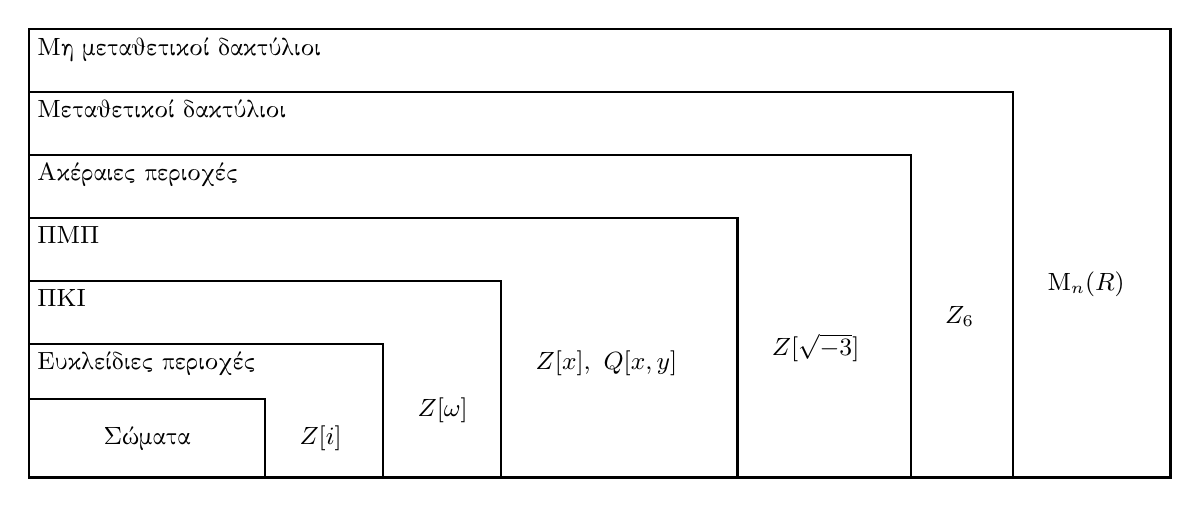
\begin{tikzpicture}[
    rect/.style={draw, thick, minimum width=3cm, minimum height=1cm, anchor=south west},
    font=\small
]

% Base rectangle
\node[rect] (fields) at (0,0) {Σώματα};

% Euclidean domains
\node[rect, minimum width=4.5cm, minimum height=1.7cm] (ed) at (0,0) {};
\node[anchor=north west] at (ed.north west) {Ευκλείδιες περιοχές};
\node[anchor=west] at ($(fields.east)+(0.3,0)$) {$\ZZ[i]$};

% PID
\node[rect, minimum width=6cm, minimum height=2.5cm] (pid) at (0,0) {};
\node[anchor=north west] at (pid.north west) {ΠΚΙ};
\node[anchor=west] at ($(ed.east)+(0.3,0)$) {$\ZZ[\omega]$};

% UFD
\node[rect, minimum width=9cm, minimum height=3.3cm] (ufd) at (0,0) {};
\node[anchor=north west] at (ufd.north west) {ΠΜΠ};
\node[anchor=west] at ($(pid.east)+(0.3,0.2)$) {$\ZZ[x],\ \QQ[x,y]$};

% Integral domains
\node[rect, minimum width=11.2cm, minimum height=4.1cm] (id) at (0,0) {};
\node[anchor=north west] at (id.north west) {Ακέραιες περιοχές};
\node[anchor=west] at ($(ufd.east)+(0.3,0)$) {$\ZZ[\sqrt{-3}]$};

% Commutative rings
\node[rect, minimum width=12.5cm, minimum height=4.9cm] (cr) at (0,0) {};
\node[anchor=north west] at (cr.north west) {Μεταθετικοί δακτύλιοι};
\node[anchor=west] at ($(id.east)+(0.3,0)$) {$\ZZ_6$};

% Noncommutative rings
\node[rect, minimum width=14.5cm, minimum height=5.7cm] (ncr) at (0,0) {};
\node[anchor=north west] at (ncr.north west) {Μη μεταθετικοί δακτύλιοι};
\node[anchor=west] at ($(cr.east)+(0.3,0)$) {$\mathrm{M}_n(\RR)$};

\end{tikzpicture}
\]
όπου $\omega = \frac{1 + \sqrt{-19}}{2}$.

Θα χωρίσουμε την απόδειξη του Θεωρήματος \ref{thm:PID_UFD} σε δύο μέρη. Πρώτα θα δείξουμε την ύπαρξη μιας παραγοντοποίησης σε ανάγωγα στοιχεία (βλ. συνθήκη $(1)$ του Ορισμού 2.11) και έπειτα την μοναδικό\-τητα ως προς αναδιατάξεις των μερών της και ως προς συντροφικό\-τητα (βλ. συνθήκη $(2)$ του Ορισμού 2.11). To πρώτο μέρος της απόδειξης βασίζεται στην παρατήρηση ότι κάθε αύξουσα ακολουθία ιδεωδών σε μια περιοχή κύριων ιδεωδών είναι τελικά σταθερή.
\begin{lemma}
    \label{lem:pid_is_noetherian}
    Έστω $R$ μια περιοχή κύριων ιδεωδών. Αν 
    \[
    I_1 \subseteq I_2 \subseteq \cdots 
    \]
    είναι μια αύξουσα ακολουθία ιδεωδών του $R$, τότε 
    \[
    I_m = I_{m+1} = \cdots 
    \]
    για κάποιο $m \ge 1$.
\end{lemma}
\begin{proof}[Απόδειξη]
    Έστω 
    \[
    I = \bigcup_{n \ge 1} I_n = I_1 \cup I_2 \cup \cdots \subseteq R.
    \]
    Το $I$ είναι ιδεώδες του $R$. Πράγματι,
    \begin{itemize}
        \item περιέχει το μηδέν (γιατί;)
        \item είναι κλειστό ως προς την πρόσθεση, διότι αν $a, b \in I$, τότε $a \in I_k$ και $b \in I_\ell$, για κάποια $k, \ell \ge 1$, τα οποία μπορούμε, χωρίς βλάβη της γενικότητας, να τα διαλέξουμε τέτοια ώστε $k \le \ell$ και γι αυτό $a \in I_k \subseteq I_\ell$. Συνεπώς $a + b \in I_\ell \subseteq I$, διότι το $I_\ell$ είναι ιδεώδες του $R$. 
        \item είναι κλειστό ως προς πολλαπλασιασμό με στοιχεία του $R$, διότι αν $a \in I$ και $r \in R$, τότε $a \in I_k$, για κάποιο $k \ge 1$ και κατά συνέπεια $ra \in I_k \subseteq I$, διότι το $I_k$ είναι ιδεώδες του $R$.
    \end{itemize}

    Επειδή όμως το $R$ είναι περιοχή κύριων ιδεωδών, έπεται ότι 
    \[
    I = (a)
    \]
    για κάποιο $a \in R$. Τότε $a \in I$ και γι αυτό $a \in I_m$, για κάποιο $m \ge 1$. Κατά συνέπεια, $(a) \subseteq I_m$, που αναγκάζει $I = (a) = I_m$ και γι αυτό 
    \[
    I = I_m = I_{m+1} = \cdots.
    \]
\end{proof}

\begin{remark}
    Γενικά, η ένωση ιδεωδών δεν είναι κατ' ανάγκη ιδεώδες. Για παράδειγμα, για $R = \ZZ$, το σύνολο $(2) \cup (3)$ δεν είναι κλειστό ως προς την πρόσθεση, διότι 
    \[
    2 + 3 = 5 \notin (2) \cup (3)
    \]
    παρόλο που $2 \in (2)$ και $3 \in (3)$.
\end{remark}

\begin{proof}[Απόδειξη του Θεωρήματος \ref{thm:PID_UFD} (Μέρος πρώτο)]
    Έστω $R$ μια περιοχή κύριων ιδεωδών και $r \in R$ ένα μη μηδενικό, μη αντιστρέψιμο στοιχείο. Θέλουμε να δείξουμε ότι μπορεί να γραφεί ως γινόμενο πεπερασμένου πλήθους ανάγωγων στοιχείων του $R$. Αν το $r$ είναι ανάγωγο, τότε τελειώσαμε. Διαφορετικά, μπορούμε να γράψουμε 
    \begin{equation}
        \label{eq:pid_is_ufd}
        r = a_1b_1 
    \end{equation}
    για κάποια $a_1\notin R^\times$ \emph{και} $b_1 \notin R^\times$. Από την Σχέση \eqref{eq:pid_is_ufd} έπεται ότι 
    \[
    (r) \subsetneqq (a_1)
    \]
    διότι αν $(r) = (a_1)$, τότε τα στοιχεία $r$ και $a_1$ θα ήταν συντροφικά, που θα σήμαινε ότι $r = ua_1$ για κάποιο αντιστρέψιμο $u \in R^\times$, το οποίο είναι αδύνατο λόγω της υπόθεσης ότι το $r$ δεν είναι ανάγωγο.

    Tώρα, σκεπτόμενοι την Σχέση \eqref{eq:pid_is_ufd}, αν τα $a_1$ και $b_1$ είναι ανάγωγα, τότε τελειώσαμε. Διαφορετικά, κάποιο από αυτά δεν είναι ανάγωγο. Χωρίς βλάβη της γενικότητας, υποθέτουμε ότι αυτό είναι το $a_1$. Τότε, μπορούμε να γράψουμε 
    \[
    a_1 = a_2b_2
    \]
    για κάποια $a_2\notin R^\times$ \emph{και} $b_2 \notin R^\times$. Όμοια με πριν, έπεται ότι 
    \[
    (a_1) \subsetneqq (a_2).
    \]

    Συνεχίζοντας αυτή τη διαδικασία κάθε φορά που ένας παράγοντας δεν είναι ανάγωγος, προκύπτει μια \emph{γνησίως} αύξουσα ακολουθία 
    \[
    (r) \subsetneqq (a_1) \subsetneqq (a_2) \subsetneqq \cdots
    \]
    ιδεωδών του $R$. Επειδή το $R$ είναι περιοχή κύριων ιδεωδών, το Λήμμα \ref{lem:pid_is_noetherian} μας πληροφορεί ότι 
    \[
    (a_m) = (a_{m+1}) = \cdots 
    \]
    για κάποιο $m \ge 1$. Αυτό είναι αδύνατο, διότι η ακολουθία που κατασκευάσαμε ήταν γνησίως αύξουσα. Συνεπώς, σε κάποιο βήμα της διαδικασίας όλοι οι παράγοντες πρέπει να είναι ανάγωγοι και το ζητούμενο έπεται.
\end{proof}

Αυτό είναι ένα παράδειγμα μη-κατασκευαστικής απόδειξης. Πιο συγκεκριμένα, δεν μας πληροφορεί πως να υπολογίσουμε την ζητούμενη παραγοντοποίηση, παρά μόνο την ύπαρξή της. Τέτοιου είδους αποδείξεις πρωτοεμφανίστηκαν στα τέλη του δέκατου ένατου αιώνα και αποτέλεσαν σημείο καμπής στην ανάπτυξη της (αφηρημένης) άλγεβρας. Εκτός αυτού, πυροδότησαν την μελέτη της συστηματικής θεμελίωσης των μαθηματικών.

Το δεύτερο μέρος της απόδειξης βασίζεται στην παρατήρηση ότι σε μια περιοχή κύριων ιδεωδών οι έννοιες ανάγωγο και πρώτο στοιχείο είναι ισοδύναμες\footnote{Θυμηθείτε την περίπτωση του δακτυλίου των ακεραίων στη συζήτηση πριν την Πρόταση 1.10.} και κατά συνέπεια μπο\-ρούμε να επιχειρηματολογήσουμε όπως και στην απόδειξη του θεμελιώδους θεωρήματος της αριθμητικής. 

\begin{lemma}
    \label{lem:in_PIDs_irreducible_equals_prime}
    Έστω $R$ μια περιοχή κύριων ιδεωδών και $p \in R$ ενα μη μηδενικό, μη αντιστρέψιμο στοιχείο. Τα ακόλουθα είναι ισοδύναμα.
    \begin{itemize}
        \item[(1)] Το $p$ είναι ανάγωγο στοιχείο του $R$.
        \item[(2)] Το $(p)$ είναι μεγιστικό ιδεώδες του $R$.
    \end{itemize}
    Ειδικότερα, σε μια περιοχή κύριων ιδεωδών ένα στοιχείο είναι ανάγωγο αν και μόνο αν είναι πρώτο.
\end{lemma}

\begin{proof}[Απόδειξη]
    Για τον δεύτερο ισχυρισμό, από την Πρόταση 2.8 γνωρίζουμε ότι σε μια ακέραια περιοχή (και κατά συνέπεια σε μια περιοχή κύριων ιδεωδών) κάθε πρώτο στοιχείο είναι ανάγωγο. Αντιστρόφως, επειδή κάθε μεγιστικό ιδεώδες είναι πρώτο\footnote{Γεγονός που ισχύει σε κάθε μεταθετικό δακτύλιο. (βλ. συζήτηση μετά την Πρόταση 1.10).}, ο πρώτος ισχυρισμός μας πληροφορεί ότι αν $p$ είναι ένα ανάγωγο στοιχείο του $R$, τότε το $(p)$ είναι πρώτο και κατά συνέπεια το $p$ είναι πρώτο στοιχείο του $R$ (γιατί;).

    Θα δείξουμε τώρα τον πρώτο ισχυρισμό. Για την κατεύθυνση $(1) \then (2)$, υποθέτουμε ότι το $p$ είναι ανάγωγο στοιχείο του $R$ και θεωρούμε ένα ιδεώδες $I$ του $R$ τέτοιο ώστε $(p) \subseteq I$. Επειδή ο $R$ είναι περιοχή κύριων ιδεωδών, έπεται ότι 
    \[
    I = (a)
    \]
    για κάποιο $a \in R$. Συνεπώς, 
    \[
    p = ab
    \]
    για κάποιο $b \in R$. Επειδή το $p$ είναι ανάγωγο έπεται ότι είτε $a \in R^\times$, είτε $b \in R^\times$. Στην πρώτη περίπτωση, έχουμε $I=R$ (γιατί;), ενώ στην δεύτερη περίπτωση έχουμε\footnote{Πράγματι, αν $b \in R^\times$, τότε $bc = 1$, για κάποιο $c \in R$ και γι αυτό $pc = abc = a$, που σημαίνει ότι $a \in (p)$ και κατά συνέπεια $I = (a) \subseteq (p)$.} $I = (p)$. Άρα το ιδεώδες $(p)$ είναι μεγιστικό.

    Για την αντίστροφη κατεύθυνση $(2) \then (1)$, υποθέτουμε ότι το $(p)$ είναι μεγιστικό ιδεώδες του $R$ και ότι $p = ab$ για κάποια $a, b \in R$. Τότε 
    \[
    (p) \subseteq (a) 
    \]
    και γι αυτό είτε $(p) = (a)$, είτε $(a) = R$. Στη δεύτερη περίπτωση, έπεται ότι $a \in R^\times$ (γιατί;). Στην πρώτη περίπτωση, έχουμε 
    \[
    a = pc
    \]
    για κάποιο $c \in R$ και γι αυτό 
    \[
    p = ab = pcb.
    \]
    Επειδή ο $R$ είναι ακέραια περιοχή, μπορούμε να \textquote{διαγράψουμε} το $p$ και να προκύψει ότι $1 = cb$ που σημαίνει ότι $b \in R^\times$. Άρα το $p$ είναι πρώτο στον $R$ και το ζητούμενο έπεται.
\end{proof}

Το Λήμμα \ref{lem:in_PIDs_irreducible_equals_prime} σε συνδυασμό με το Θεώρημα \ref{thm:PID_UFD} δίνουν μια ακόμη απόδειξη ότι το $\ZZ[\sqrt{-3}]$ δεν είναι περιοχή μονοσήμαντης παραγοντοποίησης, διότι το 2 είναι ανάγωγο (όπως είδαμε στο Παράδειγμα 2.9), αλλά δεν είναι πρώτο, διότι 
\[
2 \mid 4 = (1 + \sqrt{-3})(1 - \sqrt{-3})
\]
αλλά $2 \nmid 1 \pm \sqrt{-3}$.

\begin{proof}[Απόδειξη του Θεωρήματος \ref{thm:PID_UFD} (Δεύτερο μέρος)] 
    Έστω $R$ μια περιοχή κύριων ιδεωδών. Στο π\-ρώτο μέρος της απόδειξης, είδαμε ότι μπορούμε να το γράψουμε κάθε μη μηδενικό, μη αντιστρέψιμο στοιχείο ως γινόμενο ενός πεπερασμένου πλήθους ανάγωγων στοιχείων του $R$. Θα δείξουμε την μοναδικότητα κάνοντας επαγωγή ως προς το πλήθος των παραγόντων.

    Η περίπτωση μήκους $1$ (βάση της επαγωγής) είναι τετριμμένη (γιατί;). Έστω $n > 1$. Υποθέτουμε ότι κάθε μη μηδενικό, μη αντιστρέψιμο στοιχείο του $R$ μπορεί να γραφεί ως γινόμενο $n-1$ ανάγωγων στοιχείων του $R$ με μοναδικό τρόπο ως προς αναδιατάξεις των παραγόντων και ως προς συντροφικότητα (βλ. συνθήκη (2) του Ορισμού 2.11). 

    Έστω $r \in R$ ένα μη μηδενικό, μη αντιστρέψιμο στοιχείο τέτοιο ώστε 
    \[
    r = p_1p_2 \cdots p_n = q_1q_2\dots q_m
    \]
    για ανάγωγα στοιχεία $p_1, p_2, \dots, p_n, q_1, q_2, \dots, q_m \in R$. Από το Λήμμα \ref{lem:in_PIDs_irreducible_equals_prime}, το $p_1$ είναι πρώτο και γι αυτό 
    \[
    p_1 \mid q_j
    \]
    για κάποιο $1 \le j \le m$. Χωρίς βλάβη της γενικότητας, υποθέτουμε ότι $j = 1$. Συνεπώς, 
    \begin{equation}
        \label{eq:PID_implies_UFD_help}
    q_1 = u_1 p_1
    \end{equation}
    για κάποιο $u_1 \in R$. Επειδή όμως, τα $p_1$ και $q_1$ είναι ανάγωγα πρέπει αναγκαστικά $u_1 \in R^\times$. Οπότε, 
    \[
    p_1p_2\cdots p_n = q_1q_2\cdots q_m = u_1p_1q_2\cdots q_m = p_1u_1q_2\cdots q_m
    \]
    και επειδή ο $R$ είναι ακέραια περιοχή μπορούμε να \textquote{διαγράψουμε} το $p_1$ και να πάρουμε 
    \[
    p_2p_3\cdots p_n = u_1q_2q_3\cdots{q_m} = q_2'q_3'\cdots{q_m'},
    \]
    όπου $q_2' = u_1q_2$ και $q_i = q_i'$ για κάθε $3 \le j \le m$. Τα $q_2', q_3', \dots, q_m'$ είναι ανάγωγα και γι αυτό από την επαγωγική υπόθεση έπεται ότι $n-1=m-1$ και κατά συνέπεια $n=m$ και 
    \[
    q_{\pi(i)}' = u_ip_i 
    \]
    για κάθε $2 \le i \le n$ για κάποια μετάθεση $\pi \in \rmS\left(\{2,3,\dots, n\}\right)$ και κάποια $u_2, u_3, \dots, u_n \in R^\times$. Θέτοντας $\pi(1) = 1$, το ζητούμενο έπεται από την σχέση \eqref{eq:PID_implies_UFD_help}.
\end{proof}

\begin{remark}
Αποδεικνύεται ότι μια ακέραια περιοχή είναι περιοχή μονοσήμαντης παραγο\-ντοποίησης αν και μόνο αν ικανοποιεί τη συνθήκη (1) του Ορισμού 2.11 και κάθε ανάγωγο στοιχείο της είναι πρώτο (βλ. \cite[Θεώρημα~11.4.12]{Mpe15}).
\end{remark}
 
\begin{thebibliography}{99}
    \bibitem{Mpe15}
    Α. Μπελιγιάννης, 
    \textit{Μια Εισαγωγή στη Βασική Άλγεβρα},
    Κάλλιπος, 2015. (διαθέσιμο \href{https://dx.doi.org/10.57713/kallipos-547}{εδώ})
    %
    \bibitem{DF04}
    D. S. Dummit και R. M. Foote, 
    \textit{Abstract algebra},
    third edition, Wiley, 2004. 
\end{thebibliography}
\end{document}